\chapter[SM SysId of MIMO LTI systems with EIV noise structure]{Set-Membership Identification of MIMO LTI systems with EIV noise structure}

\begin{quotation}
    \textsf{\noindent Till now we have introduced fundamental aspects about Set-Membership Identification, we have understood why it is the most realistic approach to the SysId, and -- in order to go step by step -- we focused our attention on a specific case on which we developed the theory: \textit{SISO LTI systems with Errors-in-variables noise structure.} Our objective now is trying to generalize such results, including the case in which the system to identify is multi-input multi-output (MIMO) or nonlinear. In this chapter we treat the former topic.
    }
\end{quotation}

\noindent
Let us start introducing some general concepts and definition useful for the comprehension of the incoming topics. A \textbf{Multi-Input Multi-Output (MIMO)} Linear Time-Invariant system with $p$ inputs and $q$ outputs can be described by means of a \textit{matrix transfer function} $G(q^{-1})$ where each element represents a SISO transfer function 
\begin{equation}
    G_{ij}(q^{-1})=\frac{N_{ij}(q^{-1})}{D_{ij}(q^{-1})}
\end{equation} 
between the $j$-th input and the $i$-th output.\\
The I/O relationship of the system we want to study is defined by the following equation:
\begin{equation} \label{eq:MIMO_IO}
    \begin{bmatrix}
        y_1\\y_2\\\vdots\\y_q 
    \end{bmatrix}=\underbrace{\begin{bmatrix}
        G_{11}(q^{-1})&G_{12}(q^{-1})&\dots&G_{1p}{(q^{-1})}\\
        G_{21}(q^{-1})&G_{22}(q^{-1})&\dots&G_{2p}(q^{-1})\\
        \vdots&\vdots&\ddots&\vdots\\
        G_{q1}(q^{-1})&G_{q2}(q^{-1})&\dots&G_{qp}(q^{-1})
    \end{bmatrix}}_{G(q^{-1})}\begin{bmatrix}
        u_1\\u_2\\\vdots\\u_p
    \end{bmatrix}
\end{equation}
A block diagram representation of a MIMO system is reported below: 

\begin{figure}[h]
    \centering
    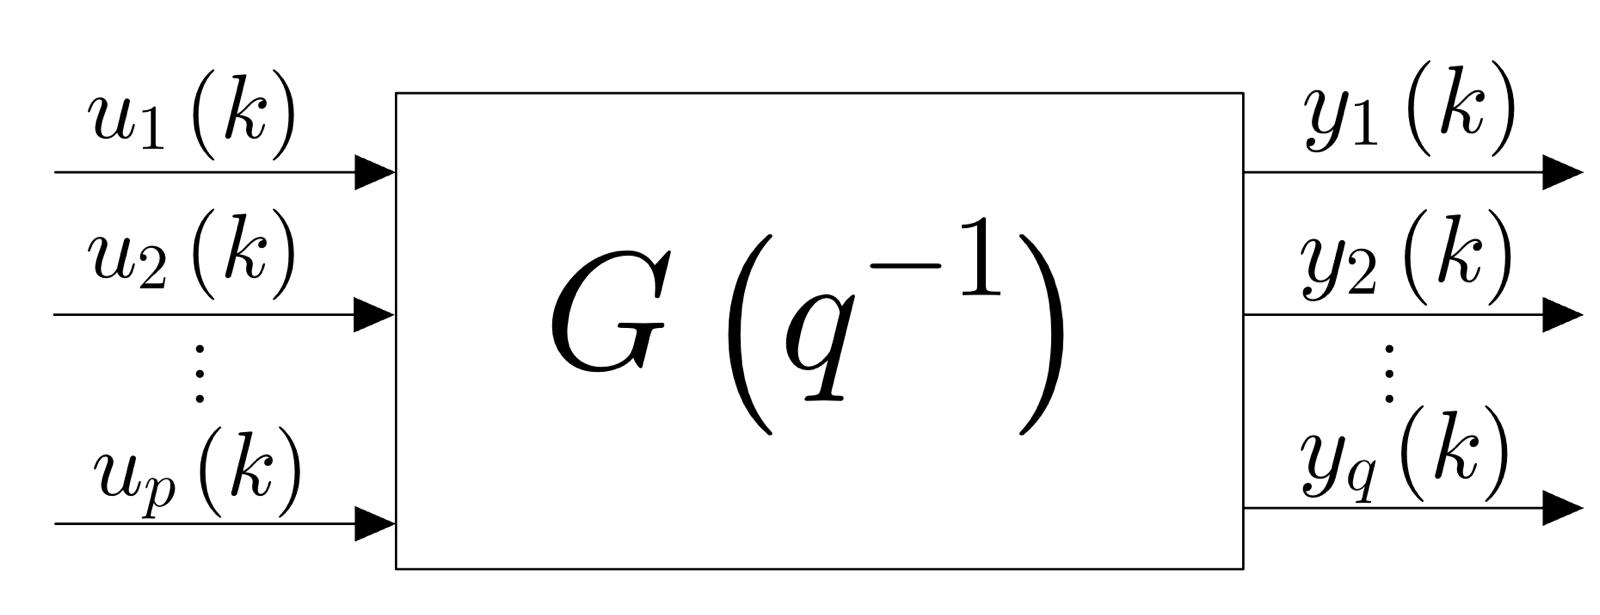
\includegraphics[scale=0.15]{img/MIMO.jpg}
    \caption{Block diagram for a MIMO system}
\end{figure}

\noindent
The reason why I use directly a transfer function description for the system I want to identify is the same for which we use it in the simple case of a SISO LTI system: since we are able to do some open-loop experiments on the plant collecting I/O data, an I/O description such as the \textit{regression form} (that leads to a transfer function) is the most convenient way to mathematically describe the system itself!\\
However, we can have an objection in the sense that we can find an (apparently) \textbf{useful insight} if we start from a state-space description, roughly speaking using the matrices $A,B,C,D$. Indeed, recalling what is the definition of (matrix) transfer function $H(s)$ obtained starting from the state space description we know that:
\begin{equation*}
    \underbrace{H(s)=C(sI-A)^{-1}{B}+D}_{\textsf{continuous time}}, \quad
    \underbrace{H(z)=C(zI-A)^{-1}B+D}_{\textsf{discrete time}} 
\end{equation*}
(From now on without loss of generality, for sake of simplicity we will use $(sI-A)$ for the explanation of what follows).
By computing the inverse of the matrix $sI-A$ we have to divide it by its determinant $\det(sI-A)$ (which is also the \textit{characteristic polynomial}). For this reason all of the elements of $H(s)$ have the same common denominator, resulting into the same parameters to be estimated! \\
Now, at the end of the day our problem is \textit{estimating some parameters} exploiting I/O experimental data. The approaches I can use in order to continue developing the theory are:
\begin{enumerate}
    \itemsep-0.3em
    \item Considering the denominators of the transfer functions \textbf{identical} how the state-space insight suggests us (this plays the role of an additive a-priori information); 
    \item Considering the transfer functions as having \textbf{different denominators} resulting in a greater number of parameters to be estimated.
\end{enumerate}

\noindent
It would be better to analyze the features for one approach and for the other. We can say that the most evident advantage in considering the same all of the denominators is that we have \textbf{less parameters} entering the identification procedure. On the other hand, in the second case we could have \textbf{some physical a-priori information} that suggest us something about the order of each transfer function, the order $n$ in general can be different from one transfer function to another. In such a case we know something directly related to the number of parameters to be estimated\footnote{
    For a system of order $n$, I have $2n+1$ parameter to estimate.
}. Apparently, we are anyway tempted to say that such an information is not lost in the first case, since there could be \textbf{zero-pole cancellations} which makes also very different the several transfer functions. However this is not true, since our collected data are affected by noise and then the parameters related to the zeros/poles are not exact. It is sufficient to think about the fact we retrieve some PUIs from the Set-Membership procedure, uncertainty is embedded into the problem. This evidence suggests us that maybe the best path to be followed is not the one that apparently makes the identification problem simpler. \textit{We will going on discussing the problem following the second approach.}\\

\noindent
Starting from the (\ref{eq:MIMO_IO}), a generic output of the system $y_i$ is given by:
\begin{equation}
    y_i(k)=G_{i1}(q^{-1})u_1(k)+G_{i2}(q^{-1})u_2(k)+\dots+G_{ip}(q^{-1})u_p(k), \quad i=1,...,q
\end{equation}
From this follows an \textbf{important remark}: each output $y_i$ depends on the past samples of the output itself and the samples of the inputs $u_1,...,u_p$ not by the other outputs. In other words the $y_i$ behaviours are \textbf{independent}. Therefore, a first conclusion can be drawn: \textit{the identifiction of a MIMO LTI system with $q$ outputs is equivalent to the identification of $q$ \textbf{MISO} (Multi-input single-output) systems}. Now, the sub-problem to be faced is:

\section{SM Identification of MISO LTI systems}
As usual in a set-membership identification procedure we have to list all of the ingredients of our problem and then put them together to obtain the feasible parameter set. This is the what we are going to do.

\subsection{A-priori information on the system}
The system order $n$ is assumed to be known moreover the I/O mapping can be expressed as follows: 
\begin{equation}
    y=G(q^{-1})\begin{bmatrix}
        u_1\\\vdots\\u_p
    \end{bmatrix} = \begin{bmatrix}
        G_1(q^{-1})&G_2(q^{-1})& \dots & G_p(q^{-1})
    \end{bmatrix}\begin{bmatrix}
        u_1\\\vdots\\u_p
    \end{bmatrix}
\end{equation}
where the function $G_i(q^{-1})$ is:
\begin{equation}\label{eq:Gi}
    G_i(q^{-1}) = \frac{
        \beta_0^i+\beta_1^i{q^{-1}}+...+\beta_{n_i}^i{q^{-n_i}}
    }{1+\alpha_1^i{q^{-1}}+...+\alpha_{n_i}^i{q^{-n_i}}
    }, \quad i=1,...,p
\end{equation}
$n_i\le{n}$ is the dynamical order of $G_i(q^{-1})$. The fact that $n_i$ could be smaller is derived from some other a-priori information, otherwise we put always $n_i=n$ for that function we do not know other insights.

\subsection{A-priori information on the noise}
With the objective of being as more general as possible, we analyze the case \textbf{errors-in-variables} (EIV) where both the inputs and the output are affected by measurement noise. A block diagram showing this set-up is given here:
\begin{figure}[h]
    \centering
    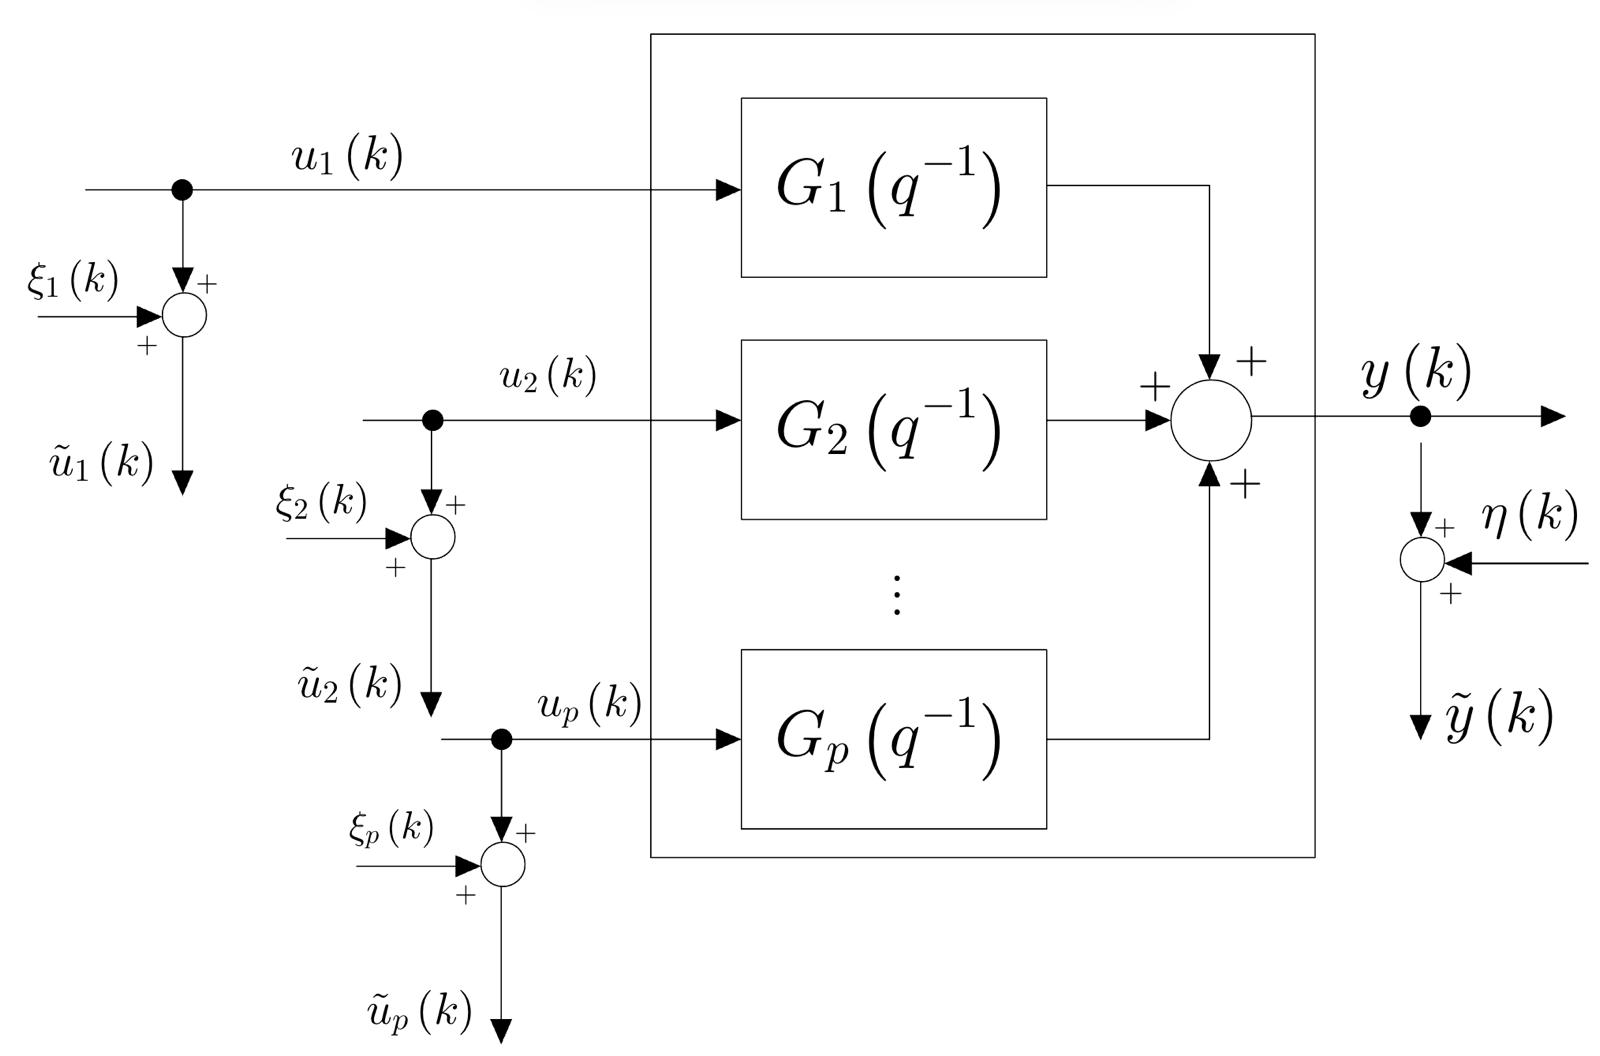
\includegraphics[scale=0.19]{img/MISO.jpg}
    \caption{Block diagram of a MISO LTI system with EIV noise structure}
\end{figure}

%TODO: figura MISO system with EIV noise structure
As in the SISO case we make some quite realistic assumptions on the boundedness of the noise samples, that is:
\begin{equation}
    \begin{aligned}
        &\vert \eta(k) \vert \le \Delta_\eta, \quad k=1,...,N\\
        &\vert \xi_i(k) \vert \le \Delta_{\xi_i} \quad k=1,...,N \quad i=1,...,p
    \end{aligned}
\end{equation}
where $N$ as usual is the number of I/O collected data, and $\Delta_{\eta}, \ \Delta_{\xi_i}$ are the only available information on the noise.

\subsection{A-posteriori information: experimental data}
In order to perform the identification $N$ samples of the inputs $\tilde{u}_1(k), ..., \tilde{u}_p(k), \quad k=1,...,N$ and the output $\tilde{y}(k)$ must be collected by doing an \textit{open-loop experiment} on the plant to be identified.

\subsection{Feasible Parameter set $\mathcal{D}_\theta$}
The next step is to put everything together in order to define the \textbf{feasible parameter set} $\mathcal{D}_\theta$:
\begin{equation} \label{eq:FPS_1}
    \begin{aligned}
        \mathcal{D}_\theta = \big\{
            \theta\in\mathbb{R}^{\sum_{i=1}^p{2n_i+1}}: \quad  
            &y(k)=G_1(q^{-1})u_1(k)+...+G_p(q^{-1})u_p(k),  \quad k=2n+1,...,N\\
            &y(k)=\tilde{y}(k)-\eta(k), \quad
            u_i(k)=\tilde{u}_i(k)-\xi_i(k), \quad i=1,...,p\\
            &
            \vert \eta(k) \vert \le \Delta_\eta, \quad \vert \xi_i(k) \vert \le \Delta_{\xi_i} \quad k=1,...,N \quad i=1,...,p
        \big\}
    \end{aligned}
\end{equation}
More explicitly we can substitute the transfer functions $G_i(q^{-1})$ with the definition we gave in (\ref{eq:Gi}), the set becomes:
\begin{equation}
    \begin{aligned}\label{eq:FPS_MIMO2}
        \mathcal{D}_\theta = \big\{
            &\theta\in\mathbb{R}^{\sum_{i=1}^p{2n_i+1}}: \quad
            y(k)={
                \frac{
                    \beta_0^1+\beta_1^1{q^{-1}}+...+\beta_{n_1}^1{q^{-n_1}}
                }{1+\alpha_1^1{q^{-1}}+...+\alpha_{n_1}^1{q^{-n_1}}
                }
            }u_1(k)+\\
            &+\dots
            +{
                \frac{
                    \beta_0^p+\beta_1^p{q^{-1}}+...+\beta_{n_p}^p{q^{-n_p}}
                }{1+\alpha_1^p{q^{-1}}+...+\alpha_{n_p}^p{q^{-n_p}}
                }
            }u_p(k),  \quad k=n+1,...,N\\
            &y(k)=\tilde{y}(k)-\eta(k), \quad
            u_i(k)=\tilde{u}_i(k)-\xi_i(k), \quad i=1,...,p\\
            &
            \vert \eta(k) \vert \le \Delta_\eta, \quad \vert \xi_i(k) \vert \le \Delta_{\xi_i} \quad k=1,...,N \quad i=1,...,p
        \big\}
    \end{aligned}
\end{equation} 
Starting from this point, how can we going on? Also in this case we could be tempted in modeling the MISO as a set of SISO, but there are some drawbacks: 
\begin{itemize}
    \item Keep in mind that for a system of order $n$ we have to solve $2(2n+1)$ optimization problems for finding the parameter uncertainty intervals, then this will result in a high computation load; 
    \item The temptation raises up from the moment that we grasp to the \textit{superposition principle for LTI systems} according which if we apply the inputs one at a time, the output will show a behaviour which is related only to that input itself. Unfortunately, in real-world applications is not always possible to "turn-off" some inputs while keeping unchanged the system, this is also because the great majority of the plants are \textit{only approximatively linear}.
\end{itemize}

\begin{comment}
Another attempt could be doing the common denominator in  (\ref{eq:FPS_MIMO2}) and solving a unique huge identification problem. Again, still there are problems! The dimension of the problem quickly would explode making unsuitable \texttt{SparsePOP} for solving the problem exploiting convex relaxation techniques. Something different is needed... 
\end{comment}

\noindent
In order to better understand the limitations behind the form (\ref{eq:FPS_1}), let us try going through the development of it. In particular, the (\ref{eq:FPS_1}) can be rewritten as: 


\begin{equation}
    \begin{aligned}
        \mathcal{D}_\theta = &\big\{
            \theta\in\mathbb{R}^{\sum_{i=1}^p{2n_i+1}}:\\
            & y(k)=\frac{
                {\color{blue}N_1({D_2 \cdot D_3 \cdot \dots D_p})} {\color{red}u_1(k)}+
                \dots+
                {\color{blue}N_p({D_1\cdot D_2 \cdot \dots D_{p-1}})} {\color{red} u_p(k)}
            }{{\color{blue}D_1 \cdot D_2 \dots D_p}}, \ k=n+1,...,N\\
            &y(k)=\tilde{y}(k)-\eta(k), \quad
            u_i(k)=\tilde{u}_i(k)-\xi_i(k), \quad k=1, ..., N \ i=1,...,p\\
            &
            \vert \eta(k) \vert \le \Delta_\eta, \quad \vert \xi_i(k) \vert \le \Delta_{\xi_i} \quad k=1,...,N \quad i=1,...,p
            \big\}=\\
            &{\color{red}=}\big\{
                \theta\in\mathbb{R}^{\sum_{i=1}^p{2n_i+1}}:\\
                &\qquad{\color{blue}(D_1 \cdot D_2 \dots D_p)} {\color{red}y(k)} = 
                {\color{blue}N_1({D_2 \cdot D_3 \cdot \dots D_p})} {\color{red}u_1(k)}+
                \dots+\\
                &\qquad +
                {\color{blue}N_p({D_1\cdot D_2 \cdot \dots D_{p-1}})} {\color{red}u_p(k)}, \ k=n+1,\dots,N\\
                &y(k)=\tilde{y}(k)-\eta(k), \quad
                u_i(k)=\tilde{u}_i(k)-\xi_i(k), \quad k=1, ..., N \quad i=1,...,p\\
            &\vert \eta(k) \vert \le \Delta_\eta, \quad \vert \xi_i(k) \vert \le \Delta_{\xi_i} \quad k=1,...,N \quad i=1,...,p
            \big\}=\\
            &{\color{red}=}\big\{
                \theta\in\mathbb{R}^{\sum_{i=1}^p{2n_i+1}}:\\
                &\qquad\big[   
                    \underbrace{(1+\alpha_1^1{q^{-1}}+\dots+\alpha_{n_1}^1q^{-{n_1}})}_{\color{blue}D_1}+\dots+
                    \underbrace{(1+\alpha_1^p{q^{-1}}+\dots+\alpha_{n_p}^p q^{-{n_p}})}_{\color{blue}D_p}
                \big] {\color{red}y(k)} =\\
                & \qquad \underbrace{(\beta_0^1 +\beta_1^1 q^{-1}+...+\beta_{n_1}^1 q^{-{n_1}})}_{\color{blue}N_1}
                \underbrace{(1+\alpha_1^2{q^{-1}}+\dots+\alpha_{n_2}^2q^{-{n_2}})}_{\color{blue}D_2} %D2
                \underbrace{(1+\alpha_1^3{q^{-1}}+\dots+\alpha_{n_3}^3q^{-{n_3}})}_{\color{blue}D_3} \dots\\
                & \qquad \underbrace{(1+\alpha_1^p{q^{-1}}+\dots+\alpha_{n_p}^p q^{-{n_p}})}_{\color{blue}D_p} {\color{red}u_1(k)}+ %D3
                \dots +  
                \underbrace{(\beta_0^p+ \beta_1^p q^{-1}+...+\beta_{n_p}^p q^{-{n_p}})}_{\color{blue}N_p}\\
                & \qquad \underbrace{(1+\alpha_1^1{q^{-1}}+\dots+\alpha_{n_1}^1q^{-{n_1}})}_{\color{blue}D_1} 
                \underbrace{(1+\alpha_1^2{q^{-1}}+\dots+\alpha_{n_2}^2q^{-{n_2}})}_{\color{blue}D_2} \dots\\  
                &\qquad \underbrace{(1+\alpha_1^{p-1}{q^{-1}}+\dots+
                 \alpha_{n_{p-1}}^{p-1}q^{-{n_{p-1}}})}_{\color{blue}D_{p-1}} {\color{red}u_p(k)} \quad k=n+1,...,N\\
                &y(k)=\tilde{y}(k)-\eta(k), \quad
                u_i(k)=\tilde{u}_i(k)-\xi_i(k), \quad k=1, ..., N \quad i=1,...,p\\
            &\vert \eta(k) \vert \le \Delta_\eta, \quad \vert \xi_i(k) \vert \le \Delta_{\xi_i} \quad k=1,...,N \quad i=1,...,p
            \big\}
    \end{aligned}
\end{equation}

where $N_i=N_i(q^{-1})$, $D_i=D_i(q^{-1})$. The notation is not so easy to read, however we have written it rigorously to understand that at the end, we can obtain a 'standard' regression form as in the 
SISO case. Then, what is the problem? Explicit computation will lead to \textbf{high order polynomial constraints} in the unknown variables:
\begin{equation}
    \begin{aligned}
    &\alpha_j^{i}, \quad i=1,...,p \quad j=1,...,n_i \\
    &\beta_j^{i}, \quad i=1,...,p \quad j=0,...,n_i\\
    &\eta(k), \xi_i(k), 
    \quad k=n+1,...,N \quad i=1,...,p
    \end{aligned}
\end{equation}
In general the computation of $PUI_{\theta_j}$ will lead us to POPs of order $n$, and whether $p$ would be high, the order of relaxation $\delta$ is going to be \textit{large} $\to$ bad news, since there will be the explosion of computational complexity and/or memory overflow because the size of data structures involved in the SDP problem -- obtained by applying convex relaxation techniques -- depends \textbf{exponentially} on the order of relaxation itself! This approach cannot be used neither for normal or large dimension identification problems. Something alternative is needed.

\subsection{Reducing the computational complexity: partial outputs $z_i$}
In order to reduce the computational complexity let us reformulate the problem by explicitly exploiting the fact that \textit{a MISO system is nothing but a collection of SISO systems}. Let us call $z_1,\dots,z_p$ the \textbf{partial outputs}, that is the output of the transfer functions $G_1,G_2,\dots,G_p$ before entering into the summing junction of the output $y(k)$:
\begin{equation*}
    z_1(k)=G_1(q^{-1})u_1(k) \quad
    z_2(k)=G_2(q^{-1})u_2(k)  \quad \dots \quad
    z_p(k)=G_p(q^{-1})u_p(k)
\end{equation*}
Now we can redefine the FPS by using such an observation obtaining:
\begin{equation}
    \begin{aligned}
        \mathcal{D}_{\theta}=\big\{
            \theta\in\mathbb{R}^{\sum_{i=1}^p{2n_i+1}}: \ 
            &\tilde{y}(k)-\eta(k) = z_1(k)+\dots+z_p(k) \ k=1,...,N\\
            &z_i(k) = \frac{N_i(q^{-1})}{D_i(q^{-1})} (\tilde{u}_i(k)-\xi_i(k)), \ i=1,\dots,p \quad k=n_i+1,...,N\\
            &\vert \eta(k) \vert \le \Delta_\eta, \quad \vert \xi_i(k) \vert \le \Delta_{\xi_i} \quad k=1,...,N \quad i=1,...,p
        \big\}
    \end{aligned}
\end{equation}
We cannot measure the samples $z_i(k)$ of the partial outputs, then such variables are unknowns. We have to look the problem into the \textbf{extended space} which includes all of the unknown variables (for the noise samples the same conclusion can be drawn). Then, let us define the\dots

\subsection{Extended feasible parameter set $\mathcal{D}_{\theta, z, \eta, \xi}$}
The \textbf{Extended feasible parameter set (EFPS)} has the following definition:
\begin{equation}
    \begin{aligned}
        \mathcal{D}_{\theta,z_1,z_2,...,z_p,\eta,\xi_1,\xi_2,...,\xi_p } = \big\{
            &(\theta,z_1,z_2,...,z_p,\eta,\xi_1,\xi_2,...,\xi_p) \in \mathbb{R}^{\sum_{i=1}^p{2n_i+1}+(2p+1)N}: \\
            &\tilde{y}(k)-\eta(k)= z_1(k)+\dots+z_p(k) \ k=1,...,N\\
            &z_i(k)=-\alpha_i^{i}z_i(k-1) -\alpha_2^{i}z_i(k-2)-...-\alpha_{n_i}^i z_{i}(k-{n_i})+\\
            &+\beta_0^{i}\tilde{u}_i(k)-\beta_0^{i}\xi(k)+...+\beta_{n_i}^{i}\tilde{u}_i(k-n_i)-\beta_{n_i}^i\xi_i(k) \\
            &i=1,...,p \quad k=n_i+1,...,N\\
            &\vert \eta(k) \vert \le \Delta_\eta, \quad \vert \xi_i(k) \vert \le \Delta_{\xi_i} \quad k=1,...,N \quad i=1,...,p
        \big\}
    \end{aligned}
\end{equation}

\noindent
Extending the parameter space we can note that the EFPS involves only \textit{bilinear constrints}, then we can pick again as minimum order of relaxation $\delta=1$, that is crucial from a computational point of view.\\
Now, we are adding all the samples of $z_1,...,z_p$ into the definition of the set. In principle we know that for a generic POP, the computational complexity depends \textit{exponentially also on the optimization variables}. However, even in this case can be proved that the problem of \textit{SM-ID of LTI MIMO systems with EIV noise structure} has the nice \textit{running intersection property}. This is the reason why we can use \textit{sparse convex relaxation techniques} which leads the computational complexity depending only \textbf{linearly} on the number of optimization variables.

\subsection{PUI computation for MISO LTI systems}
We have to solve a number $n_\theta=2\big(\sum_{i=1}^p{2n_i+1}\big)$ optimization problems of the form:

{\normalsize{
    \begin{equation}
        PUI_j =[\underline{\theta}_j,\ \overline{\theta}_j], \quad \underline{\theta}_j = \min_{{\theta, z, \eta, \xi} \in\mathcal{D}_{\theta, z, \eta, \xi}} \theta_j, \quad
        \overline{\theta}_j = \max_{{\theta, z, \eta, \xi} \in\mathcal{D}_{\theta, z, \eta, \xi}} \theta_j, \quad 
        j=1,...,n_\theta
    \end{equation}
}}
\noindent
The problem can be properly formulated using suitable data structures of \texttt{SparsePOP}. This is the end of the fundamental theoretical aspects of SM-ID of MIMO systems with EIV noise structure.

\section*{References}
\begin{itemize}
    \item[\Large{\ding{45}}]  \Citeauthor{cerone2018set}, \textit{\citetitle{cerone2018set}}, \citedate{cerone2018set}
\end{itemize}

